\documentclass[OPS,authoryear,toc]{lsstdoc}
\input{meta}

% Package imports go here.
\usepackage{graphicx} 

% Local commands go here.

%If you want glossaries
%\input{aglossary.tex}
%\makeglossaries

\title{Migration Plan for Construction Project Documentation to Operations}

% Optional subtitle
% \setDocSubtitle{A subtitle}

\author{%
Matthew Rumore, Leanne Guy
}

\setDocRef{RTN-076}
\setDocUpstreamLocation{\url{https://github.com/lsst/rtn-076}}

\date{\vcsDate}

% Optional: name of the document's curator
% \setDocCurator{The Curator of this Document}

\setDocAbstract{%
The Rubin Documentation Working Group proposed a documentation strategy mapping a
pathway from the Project’s documentation state to the final deliverable documentation that will become part of the record of completeness and ready for Operations.  This proposal is described in \citeds{SITCOMTN-014}. This technote proposes propose a workflow, implementation plan and timeline to migrate Project documentation deliverables to conform with the documentation strategy described in \citeds{SITCOMTN-014}.  It responds to charge items 5 and 6 in the Charge to the Documentation Working Group \citeds{LSE-489}.
}

% Change history defined here.
% Order: oldest first.
% Fields: VERSION, DATE, DESCRIPTION, OWNER NAME.
% See LPM-51 for version number policy.
\setDocChangeRecord{%
  \addtohist{1}{2024-02-20}{First draft, split out from SITCOMTN-014}{Leanne Guy,Matthew Rumore}
}

\graphicspath{{figures/}} %Setting the graphicspath

\begin{document}

% Create the title page.
\maketitle
% Frequently for a technote we do not want a title page  uncomment this to remove the title page and changelog.
% use \mkshorttitle to remove the extra pages

% ADD CONTENT HERE
\section{Introduction}

\subsection{Scope}

This document fully addresses charge items 5 and 6 and partially addresses charge item 7 in the Charge to the Project-Wide Documentation Working Group \citeds{LSE-489}. 

\textbf{Charge Item 5}: The working group shall propose a workflow, implementation plan and timeline to migrate Project documentation deliverables to conform with the documentation strategy in 3. The timeline should envisage completion of implementation prior to the end of
construction and handoff to operations. A distinction shall be made between static controlled documents and those that are intended to evolve in time through the end of
construction and into operations.

\textbf{Charge Item 6}: Based on required input from each subsystem, SIT-COM and the Project Office, the working group shall provide an assessment of the resources needed to meet the objectives defined by items 2, 3 and 4. This includes resources for implementation and population of data into a system. This includes personnel, contracted services (if necessary) and system procurements.

\textbf{Charge Item 7}: The working group shall provide a risk assessment for not meeting requirements for
each tier in the document package.

\section{Transition Plan and Workflow}

Describe the process for transition from the current state to the future state.

Design a workflow

\section{Required Resources \& Subsystem Responsibilities}

Description of the estimated resources need to carry out this implementation plan and what the roles and responsibilities are for each subsystem in this context.

Need to take information from Storage View subsections, then find gaps to confirm add with DWG or identify potential gaps for project/departments/groups to consider.

The departments and technical groups are responsible; documentation specialists primary assistants; and both depend on system administrators and software developers on case-by-case need.
Transition Joint Work.

\begin{enumerate}
        \item Documentation Quantification
        \item Documentation Selection
        \item Proposed repositories Reviewing
        \item Starting and Finishing Scheduling
\end{enumerate}

Recommend new Operations Documentation Committee/Group for project-wide support, common tools and distributed development of them, lessons learned, etc.
Project-provided charge and scope.
Composition: documentation lead(s), documentation specialists, SQuaRE seat, ex-officio manager (department or subgroup?)
Need Chuck, Austin, Leanne input to min (and possibly max) bound level of effort for this role.

\begin{figure}[t]
\caption{Temporary Caption.}
\centering
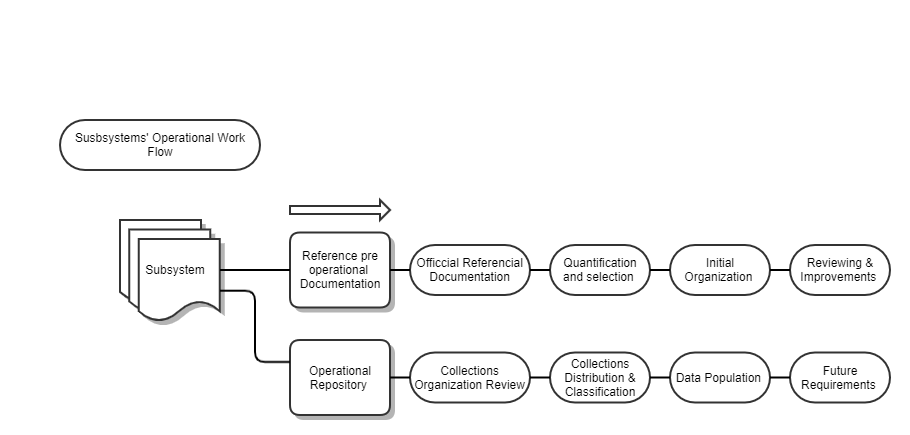
\includegraphics[width=\textwidth]{subsystems-role-workflow-temp}
\label{fig:subsystems-role-workflow}
\end{figure}

\begin{figure}[t]
\caption{Temporary Caption.}
\centering
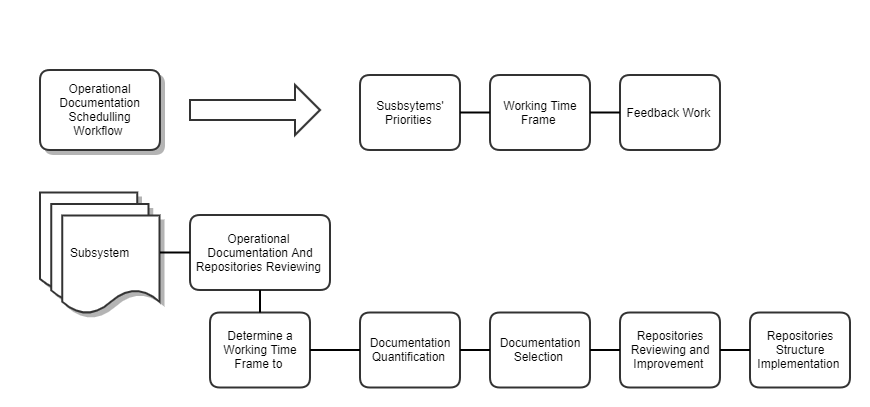
\includegraphics[width=\textwidth]{scheduling-workflow-temp}
\label{fig:scheduling-workflow}
\end{figure}

%%% Schedule  
\section{Schedule}

Outline the schedule needed for implementation to meet the objective delivering a coherent tachnical document packed at the end of the Project Construction effort.
Need to take information from Storage View subsections, then find gaps to confirm add with DWG or identify potential gaps for project/departments/groups to consider.


%%% Risk
\section{Risk Analysis}

A full risk assessment is not provided here, rather a few high-level observations on the risk of not meeting requirements id provided. A full risk analysis will be carried out following the processes and procedures of the Rubin Risk Board.


Add in a high level risk analysis with maybe some overarching risk considerations. 
State that risks will be developed and added to the Rubin Risk Register following  the procedures outlined in \citeds{rdo-71}.

Describe the risk exposure if various part of the whole of this implementation is not conducted.

Once rest of report is in good draft form, meet with Chuck after preliminary outline is available.
Some information in other portions of report.
IF, THEN statements needed?

Create at least one project managed risk; confirm if should remain the worst offender or some sum-of-parts roll-up.
Are non-project managed risks managed by someone else, or just historical justification background?



\appendix

% \input{AppendixExamples}

% Include all the relevant bib files.
% https://lsst-texmf.lsst.io/lsstdoc.html#bibliographies
\section{References} \label{sec:bib}
\renewcommand{\refname}{} % Suppress default Bibliography section
\bibliography{local,lsst,lsst-dm,refs_ads,refs,books}

% Make sure lsst-texmf/bin/generateAcronyms.py is in your path
\section{Acronyms} \label{sec:acronyms}
\addtocounter{table}{-1}
\begin{longtable}{p{0.145\textwidth}p{0.8\textwidth}}\hline
\textbf{Acronym} & \textbf{Description}  \\\hline

DM & Data Management \\\hline
\end{longtable}

% If you want glossary uncomment below -- comment out the two lines above
%\printglossaries


\end{document}
